% !TeX spellcheck = en_GB
\documentclass[a4paper]{report}
\usepackage[T1]{fontenc}
\usepackage[utf8]{inputenc}
\usepackage[english]{babel}
\usepackage{geometry}
\usepackage{graphicx}
\usepackage{subfig}
\usepackage{fancyvrb}
\usepackage{tikz}
\usetikzlibrary{calc}

\usepackage{color}
\usepackage{listings}
\lstset{ %
	language=C++,                % choose the language of the code
	basicstyle=\footnotesize,       % the size of the fonts that are used for the code
	numbers=left,                   % where to put the line-numbers
	numberstyle=\footnotesize,      % the size of the fonts that are used for the line-numbers
	stepnumber=1,                   % the step between two line-numbers. If it is 1 each line will be numbered
	numbersep=5pt,                  % how far the line-numbers are from the code
	backgroundcolor=\color{white},  % choose the background color. You must add \usepackage{color}
	showspaces=false,               % show spaces adding particular underscores
	showstringspaces=false,         % underline spaces within strings
	showtabs=false,                 % show tabs within strings adding particular underscores
	frame=single,           % adds a frame around the code
	tabsize=2,          % sets default tabsize to 2 spaces
	captionpos=b,           % sets the caption-position to bottom
	breaklines=true,        % sets automatic line breaking
	breakatwhitespace=false,    % sets if automatic breaks should only happen at whitespace
	escapeinside={\%*}{*)}          % if you want to add a comment within your code
}

\geometry{a4paper,top=2.5cm,bottom=2.5cm,left=3cm,right=3cm,%
	heightrounded,bindingoffset=5mm}
\begin{document}
	
\begin{titlepage}

	\begin{tikzpicture}[overlay,remember picture]
		\draw[line width=4pt]
		($ (current page.north west) + (1cm,-1cm) $)
		rectangle
		($ (current page.south east) + (-1cm,1cm) $);
		\draw[line width=1.5pt]
		($ (current page.north west) + (1.2cm,-1.2cm) $)
		rectangle
		($ (current page.south east) + (-1.2cm,1.2cm) $);
	\end{tikzpicture}
	
	\begin{center}
		\textup{\large  \textbf{University of Pisa}\\[0.5cm]\textbf{\large M.Sc IN COMPUTER ENGINEERING}}
		
		%---------------------------------Figure------------------------------
		\vspace{\stretch{1}}
		\begin{center}
			\begin{figure}[h]  %h means here other options t , b, p, etc.
				\centering
				
\includegraphics[width=0.3\linewidth]{./img/unipi.png}
			\end{figure}
		\end{center}
		
		%----------------------------
		\begin{LARGE}
			{\textbf {"LINEAR FEEDBACK SHIFT REGISTER" }}\end{LARGE}\\[1cm]
		\textit{AUTHOR}\\[0.1cm]
		\begin{Large}
			\textbf{Francesco Iemma}\\[0.1cm]
		\end{Large}
		
		
		\vfill
		\vspace{\stretch{2}}
		\textbf{Academic Year: 2020/2021}
	\end{center}

\end{titlepage}

%\title{\Huge{Linear Feedback Shift Register}}
%\author{\Large{Francesco Iemma}}
%\date{Academic Year 2020/21}
%\maketitle
\tableofcontents

\chapter{Introduction}
The Linear Feedback Shift Register (LFSR) is a shift register \footnote{A shift register is a sequential logic circuit made up of  chain of flip flops, for each rising edge of the clock the value of each flip-flop is shifted to the next flip-flop} in which some bits are manipulated and fed back to the input in order to generate, thanks to the shifting, a sequence of bits. So we can say that its input is the output of a linear function of its previous state.

\noindent The initial value of the LFSR is the so-called seed and it affects the stream of bits generated by the LFSR. However, this stream is not (obviusly) really random because the number of possible states is finite and the stream of bits is determined by its current or previous state and, moreover, is possible to compute the bit generated knowing the seed and the feedback function.
\noindent Anyway if the feeback function is well-choosen then the LFSR can produce a sequence of bits that appears random and which has a very long cycle, so this means that the output starts to repeat the generated numbers after a very long time. So we can assume, at least within a cycle, that it generates random numbers. For this reason the sequences generated from an LFSR are called pseudo-random.

\section{Algorythm Description}
In order to understand the LFSR algorythm we need to discuss about the \emph{feedback function}: it is the function which describes the way in which some spefic bits of the shift register are manipulated and then fed back to the input. Usually the arrangment of the inputs of the feedback function is represented as polynomial mod 2. In our case the feedback polynomial is:
\[1+x^{11}+x^{13}+x^{14}+x^{16}\]
Analysing the polynomial we can understand how LFSR works. In particular the feedback polynomial indicates which bits of the shift register affects the next state, these are called \emph{taps}.
In most cases the way in which the taps affect the next state is using XOR gates (but also XNOR gates can be used).

\noindent Now let's assume that we have an LFSR with a length of N and see how it works. At the starting state in the LFSR we have the seed. Then the feedback logic starts to work and the bit released from this logic is the new $0^{th}$ bit and the others bits are shifted by one to the right and due to the shift the previous last bit, i.e. the $(N-1)^{th}$ which has become\footnote{with $N^{th}$ we indicate the bit which is out of the LFSR. A shift register with a length of N has N bits and so its bits are the ones in the interval [0, N-1], the  $N^{th}$ doesn't exist but it's a way to indicate the "overflow" bit.} the $N^{th}$, will be the output of the LFSR.

\noindent In a more formal way (let's assume $b'_i$ the i-th old bit, $b_i$ the i-th new bit, N the length of LFSR with $N>0$, $T$ the set which contains the indexes of the taps and $y$ the function which represents the feedback logic) I can say:
\begin{itemize}
	\item $b_0 = y(b'_j, ..., b'_k)$ where  $j, ..., k \in T$
	\item $b_i = b'_{i-1}$  for $1\leq i<N$
	\item $output = b'_{N-1}$
\end{itemize}

\noindent The taps in our case are the bits 11, 13, 14, 16 (we can recognize them gazing to the exponents of \emph{x} in the feedback polynomial) so this means that the inputs of the feedback logic are these. And so in our previous notation $T=\{11, 13, 14, 16\}$, then $b_0 = y(11, 13, 14, 16)$.

\noindent In the following image it's possible to see a logic representation of a generic LFSR.
\begin{figure}[htbp]
	\centering
	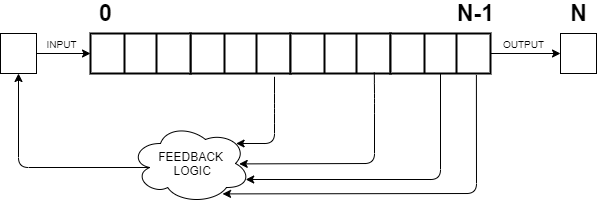
\includegraphics[scale=0.5]{img/LFSR-functionality.png}
	\caption{Logic representation of a LFSR}
\end{figure}
\section{LFSR's Properties}
In order to complete this brief journey through the world of LFSRs, let focus on a particular type of LFSR which has an interesting property, this is the so-called maximum-length LFSR. An LFSR is a maximum-length one, if and only if, the feedback polynomial is primitive and so it's necessary that:
\begin{itemize}
	\item The number of taps is even
	\item The taps values are coprime
\end{itemize}
The property of a maximum-length LFSR is the following: if its length is N then it will assume all the possible $2^N-1$ states (the state with all 0 is excluded because otherwise it will stop).

\noindent Others properties for generic LFSRs are:
\begin{itemize}
	\item As we can saw previously, the output is deterministic, in fact it's possible to compute it starting to the current state
	\item The state with all zeroes is not allowed, for this reason even a maximum-length LFSR cannot generate a sequence of $2^N$ states
\end{itemize}
It's important to point out that even if the output is deterministic the LFSRs are spreadly used, this happens because some techniques can be adopted to resolve this issue, for example giving an irregular clock to the device or manipulating the output stream with some non-linear combination of two or more bits extracted from this stream.

\section{Possible Applications}
LFSRs are spreadly used in a lot of fields. Let's see the most important ones:
\begin{itemize}
	\item They are used in Criptograhpy as pseudo-random number generators for stream-chipers (especially in military applications). In this field it's very important to resolve the issue about the deterministic behaviour of the LFSR in order to avoid possible attacks, some possible strategies are the ones seen in the previous section.
	\item They are used in Communication, for example in the Global Position System (GPS) and also in radio-jamming in order to generate a pseudo-random noise. Then another application in this field is for scrabbling, the bits produced from an LFSR are combined with the data bit in order to have a convenient stream of data that ensures good properties and better performance from the viewpoint of the modulator/demodulator. Then it is also used in CRC (Cyclic Redundancy Check).
	\item They are used in Electronics in order to do a pseudo-random testing of a circuit in order to test "all" possibile inputs of the circuit (in fact this technique is also called pseudo-exhaustive testing)
\end{itemize}


\section{Possible Architectures}
There are two type of possible LFSR's architectures:
\begin{itemize}
	\item Fibonacci LFSR (also called "Many-To-One architecture", because from "many" bits you obtain "one" bit that is the new input bit)
	\item Galois LFSR (also called "One-To-Many architecture", because from "one" bit - that is the last one and also the output - you obtain "many" bits that are the ones which are in positions next to the taps)
\end{itemize}
\begin{figure}[htpb]
	\centering
	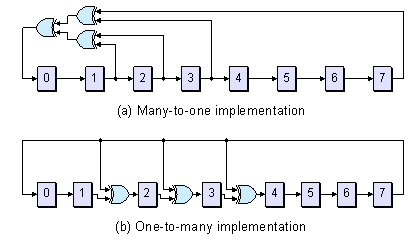
\includegraphics[scale=0.9]{img/architectures.png}
	\caption{LFSR Architectures - Source: www.eetimes.com}
\end{figure}
\subsection{Fibonacci LFSR}
The Fibonacci LFSR is the simplier possible architecture for an LFSR  and it is also the standard one, basically the generical things said so far about LFSRs describe the Fibonacci LFSR. In fact, for instance, we can observe that the figure 1.2.(a) and the figure 1.1 are indeed the same figure with the difference that the 1.1 is a logic representation and so the gates have not been drawn (they are in the so-called "Feedback Logic").
\subsection{Galois LFSR}
The Galois LFSR is an alternative architecture for LFSR, from the point of view of the output it's equivalent to Fibonacci one (the output of a Galois it's the same of a Fibonacci) but indeed they are internally different. On the rising edge of the clock, all bits that are not taps are shifted unchanged to the right by one position. Instead the taps are XORed with the previous last bit and the output of this XOR operation goes to the next bit on the right. In a more formal way we can write (let's assume $b'_i$ the i-th old bit, $b_i$ the new i-th bit, N the length of LFSR with $N>0$, $T$ the set which contains the indexes of the taps):
\begin{itemize}
	\item $b_0 = b'_{N-1}$
	\item $b_{i+1} = b'_i$ with $i\notin T$ , $0\le i < N-1$
	\item $b_{j+1} = XOR(b'_{N-1} , b_j)$ with $j \in T$ , $0\le j < N-1$
	\item $output = b'_{N-1}$
\end{itemize}
\subsection{Comparison}
The Galois architecture has a big advantage with respect to Fibonacci one. In fact in the latter there is a chain of XOR gates and the XOR operations must be done in serial and it cannot be done in parallel. Furthermore, the propagation time of this chain is not negligible. On the other hand, in the Galois implementation, the XOR operations can be done in parallel and the propagation time regard a single gate (not a chain as in the Fibonacci's case). So the propagation time of Galois implementation is lesser than the Fibonacci one, this means that with this architecture we can achieve a faster clock frequency.
In our case we have four taps, so if we assume that we have only XOR gates with two inputs and each one has a $t_{propagation_{i}} = x$ we are in the following situation:
	\begin{itemize}
		\item Fibonacci: we have to use three XOR gates (installed as we can see in the following image) and so the minimum clock period $T$ is equal to $T = t_{propagation_{1}} + t_{propagation_{2}} = 2x$. Then the maximum frequency achievable is $f=1/T=1/2x$. If $x=4ns$ then $f = 125 MHz$
		\begin{figure}[htpb]
			\centering
			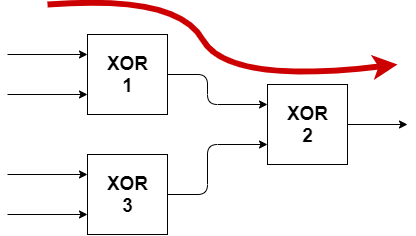
\includegraphics[scale=0.5]{img/XOR chain.png}
			\caption{Critical path (in red) related to XOR gate in Fibonacci with 4 taps}
		\end{figure}
		\item Galois: also in this case we use three XOR gates, but in this case each one is installed between two flip-flop so the critical path is made up of one gate. Then $T = t_{propagation_{1}} =x$ and so $f = 1/T = 1/x$. If $x=4ns$ then $f = 250 MHz$.
			\begin{figure}[htpb]
			\centering
			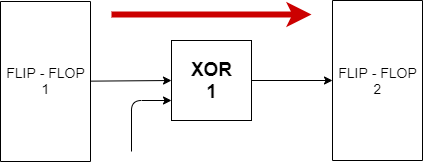
\includegraphics[scale=0.5]{img/XORtp.png}
			\caption{Critical path (in red) related to XOR gate in Galois}
		\end{figure}
	\end{itemize}
\noindent We can see that in this case $f_{Galois}=2f_{Fibonacci}$ but if the number of taps increase we have a larger difference, for example with $NumTaps = 8$ I have $f_{Galois} = 3f_{Fibonacci}$, with $NumTaps=16$ then $f_{Galois} = 4f_{Fibonacci}$. So if $NumTaps$ is a $2^a$ then $f_{Galois} = af_{Fibonacci}$.

\noindent This results shown as the Galois implementation is better from the viewpoint of the maximum clock frequency.

\noindent This difference is bigger when the number of taps grows, in most application this difference is not so evident as in the example shown and, at the end of the day, the performance are more or less the same. For example if we use XOR gate with more inputs than two the $t_{propagation}$ of Fibonacci is less than the one in the case of a cascade of XOR with two inputs. So the relation with Galois is not so unbalanced. Then in some FPGA are used LUTs that support 6 input logic function, so using a XOR with two inputs or a XOR with six is basically the same.

\noindent Indeed, theoretically speaking, the difference in performance between the two implementations exists, and so in the following report it will be treaten the implementation in VHDL of an LFSR with Galois architecture and then its testing and its practical realization obtained by programming the ZyBo Board with Xilinx Vivado. 

\chapter{Architecture Description}
As we discussed in the previous chapter, we will implement a Galois LFSR. Let's see the necessary devices to implement it.
In order to implement a memory element I need a D Flip-Flop with set and reset. In fact we need to initialize each memory element to the seed value, so the i-th flip flop will be initialize with the i-th bit of the seed.
The aim of the implementation is to have a functional LFSR, but another aim is also having a customizable LFSR. In order to do this we have to add a circuit to change (or not) the input of a simple flip-flop, we call this circuit \emph{tap circuit}.
\section{D Flip-Flop with tap circuit}
Assume that we have the i-th flip-flop and the j-th (with $j = i +1$). If $i$ is a tap then its output must be XORed with the $N-1$ bit, otherwise the output of $i$ goes unchanged to the input of $j$. So we have to implement the following logic function (described using a pseudo-code and assuming that $feedback$ is the $N-1$ bit):
\begin{lstlisting}
	void logicFunctionOmega(isTap_i, feedback)
	{
		if(isTap_i==true)
			input_j = xor(output_i,feedback);
		else
			input_j = output_i;
	}
\end{lstlisting}
Now we have to translate this logic function from this pseudo-code to logic gates.
But, before doing this, we need to point out some concepts:
\begin{itemize}
	\item $isTap_i$, $feedback$ and $output_i$ are bits. We will use the following convention: $isTap_i$ is true if it is 1, it is false when it is 0.
	\item We know that the neutral element for the XOR is the 0 (if A and B are the inputs of XOR, if B is 0 then A passes the gate unchanged), in fact the truth table for the XOR is:
	\begin{figure}[htpb]
		\centering
		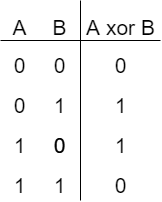
\includegraphics[scale=0.6]{img/XORtruthTable.png}
		\caption{XOR Truth Table}
	\end{figure} 
\end{itemize} 
After fixed this points we can implement our unknown function, let's call it $\Omega$ and let see what is the expected truth table (in the image A is $isTap_i$ and B is $feedback$):
\begin{figure}[htpb]
	\centering
	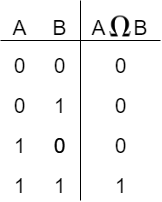
\includegraphics[scale=0.6]{img/ANDtruthTable.png}
	\caption{$\Omega$ Truth Table.}
\end{figure}

\noindent Remember that the output must be equal to B ($feedback$) if A($tap_i$) is equal to 1, otherwise it must be equal to the neutral element of the xor, so 0.

\noindent We can easily recognize that the "mysterious" logic function $\Omega$ is indeed the AND gate.
So the logic block diagram of a flip-flop with the tap circuit is the following:
\begin{figure}[htpb]
	\centering
	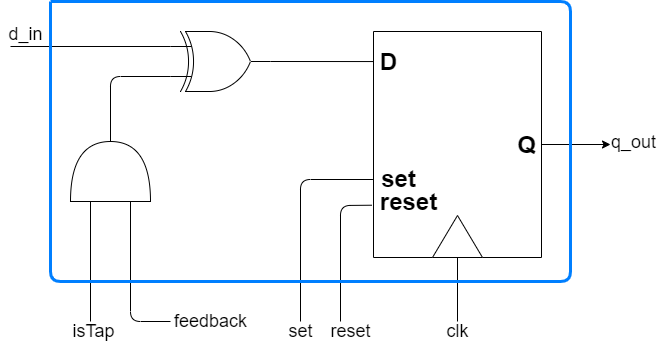
\includegraphics[scale=0.6]{img/FF_tap_circuit.png}
	\caption{Logic block diagram of a D Flip-Flop with set/reset and tap circuit.}
\end{figure}

\section{LFSR Implementation}
Once we have the D Flip-Flop with the tap circuit if we want to implement a LFSR with a length of N, we need N D Flip-Flop with tap circuit.
\begin{figure}[htpb]
	\centering
	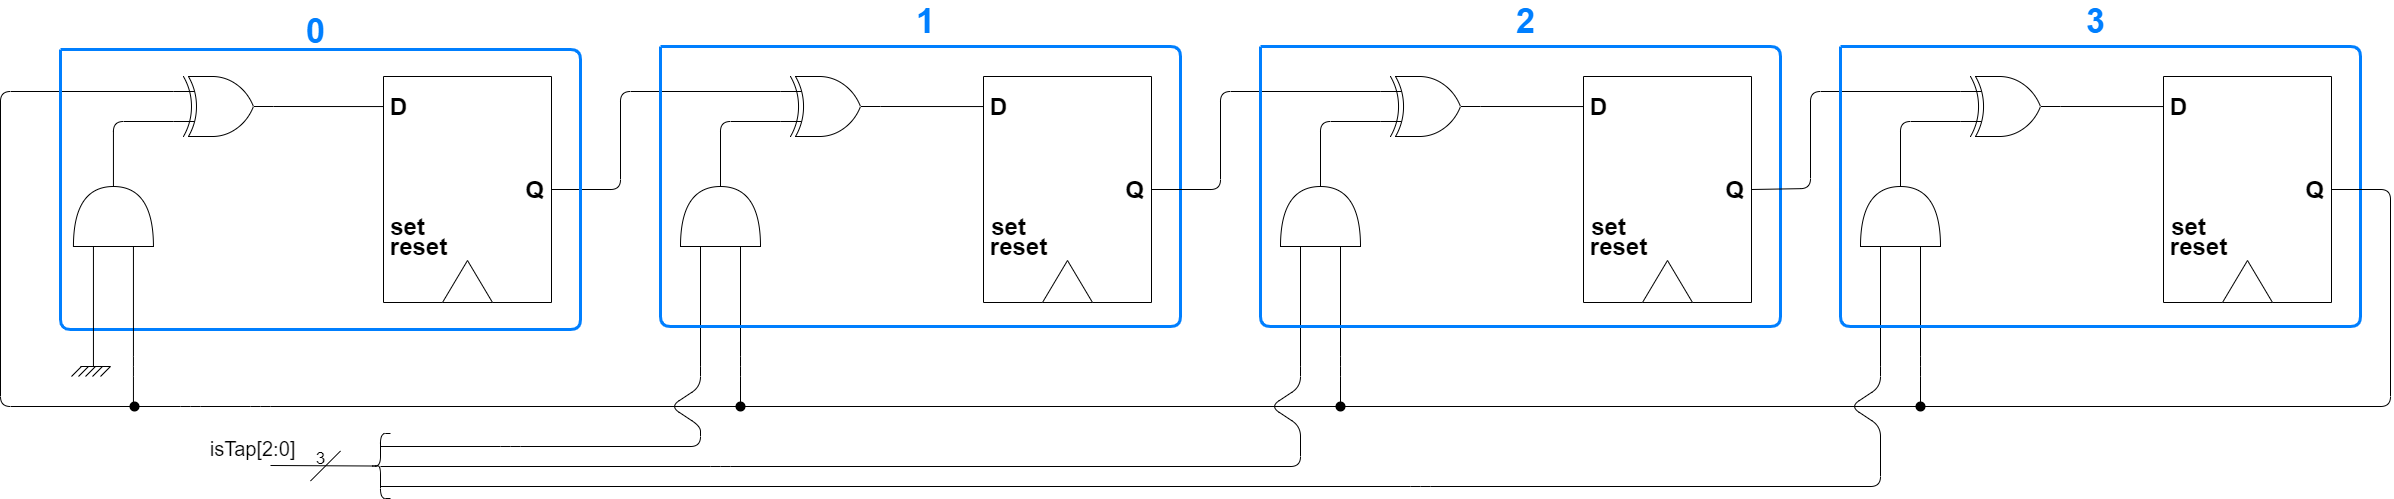
\includegraphics[scale=0.18]{img/LFSR_logic_block.png}
	\caption{Implementation of a LFSR (length of 4) with D Flip-Flop with tap circuit. (For simplicity we neglect the links for clock and set/reset)}
\end{figure}

\noindent It's important to do some observations about this implementation.
\begin{itemize}
	\item The first flip flop (the $0^{th}$) is a particular one. Its input port "isTap" must be linked to the ground (it must be always 0) because doesn't exist a flip flop before the zero one.
	\item The initialization of the flip-flops is ensured by the basic D Flip-Flop linking the set port of the $i^{th}$ flip-flop to $seed[i]$ (this is not shown in figure 2.4)
\end{itemize}

\section{Input/Output and Overall}
Abstracting from the internal details it's possible to describe the LFSR as in the image 2.5.
\begin{figure}[htpb]
	\centering
	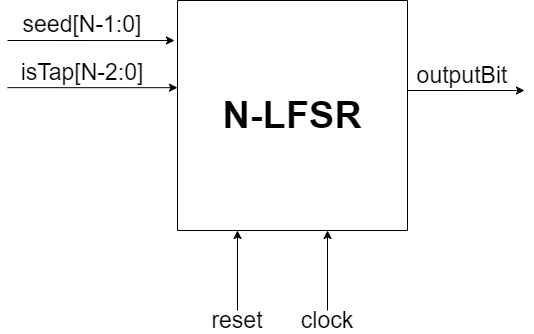
\includegraphics[scale=0.5]{img/LFSR-overall.png}
	\caption{Logic block diagram of a LFSR with a length of N.}
\end{figure}

\noindent Let's analyse the input/output ports:
\begin{itemize}
	\item \emph{seed[N-1:0]}: it contains the initialization value of the LFSR (the so-called seed). As we said previously the $i-th$ set port of the flip-flop will be connected to $seed[i]$.
	\item \emph{isTap[N-2:0]}: it indicates which are the taps. Its length is N-1 because there is no flip-flop before the $0^{th}$ flip-flop and so its isTap port will be connected to the ground (zero).
	\item \emph{reset}: the reset in common for all flip-flops.
	\item \emph{clock}: the clock in common for all flip-flops.
	\item \emph{outputBit}: the bit that is the result of the LFSR's algorithm.
\end{itemize} 
Let's sum up the operations done by the LFSR:

\noindent The LFSR is programmable, because once we have fixed the length N it can works with any polynomial feedback because of \emph{isTap[N-2:0]}. Then it's also possible to initialize, at the reset, the shift register using \emph{seed[N-1:0]}. Then, when all these signal are given to the device, it start to work and to produce a pseudo-random sequence of bits.
\chapter{VHDL Code}
In this section we will see the VHDL code for all the devices seen previously: starting from the basic ones, that are necessary to implement an LFSR, to arrive at the LFSR itself.
\section{D Flip-Flop with Set/Reset}
The basic device needed for the LFSR is a D Flip-Flop wit Set/Reset.
\lstset{ %
	language=VHDL}
\begin{lstlisting}
	-- D Flip-Flop with Set/Reset
	library ieee;
	use ieee.std_logic_1164.all;
	
	entity dff is
		port(
			clk		:	in 	std_logic;
			reset	:	in 	std_logic;
			set 	:	in 	std_logic;
			d 		:	in 	std_logic;
			q 		:	out std_logic
		);
	end dff;
	
	architecture rtl of dff is
	begin
		dff_p:process(reset,clk)
		begin
			if reset='0' then
				q <= set;
			elsif(rising_edge(clk)) then
				q <= d;
			end if;
		end process;
	end rtl;
\end{lstlisting}
The behaviour of this device is very simple, at the initialization phase (when reset is 0) the output is initialized with the set value. Then in the normal case the output follow the input and it is update at each rising edge of the clock.

\section{D Flip-Flop with Set/reset and Tap Circuit}
The memory cell which maintains a bit within the LFSR is the D-Flip-Flop with Set/Reset and tap circuit that implements the characteristic features of the LFSR which differentiates it from a simple shift register.
\begin{lstlisting}
	-- D Flip-Flop with Set/Reset and tap circuit
	library ieee;
	use ieee.std_logic_1164.all;
	
	entity dff_tap_circuit is
		port(
			clk				:	in 	std_logic;
			reset 		:	in 	std_logic;
			set				:	in 	std_logic;  -- initialization input
			d_in			:	in 	std_logic;	
			isTap			:	in 	std_logic;	-- it indicates if the input must be changed
																	-- (it does if the previous ff is a tap)
			feedback	:	in 	std_logic;  -- it is the feedback bit (the N-1)
			q_out			:	out std_logic
		);
	end dff_tap_circuit;
	
	
	architecture rtl of dff_tap_circuit is
	component dff is
		port(
			clk		:	in 	std_logic;
			reset :	in 	std_logic;
			set		:	in 	std_logic;
			d 		:	in 	std_logic;
			q 		:	out std_logic
		);
	end component;
	
	signal new_d : std_logic;
	begin
		internal_dff : dff
		port map(
			clk 	=> clk,
			reset	=> reset,
			set 	=> set,
			d 		=> new_d,
			q 		=> q_out
		);
		
		new_d <= d_in xor (isTap and feedback);
	
	end rtl;
\end{lstlisting}
This device acts as the previous, the only difference is the addition of the tap circuit which is described in the row 41.

\section{LFSR}
Now we see the way in which we have to aggregate the previous devices in order to implement an LFSR.

\noindent We use (0 to N) instead of (N downto 0) in the declaration of the standard logic vectors for isTap and seed, because they are not numbers but they indicate positions, so the left-most bit is the one for the $0^{th}$ flip-flop and so in order to access it I would like to use the following notation: \emph{vector(0)} and not this \emph{vector(N-1)}. To achieve this aim I have to use the keyword \emph{to} instead of \emph{downto}.
\begin{lstlisting}
-- LinearFeedbackShiftRegister
library ieee;
use ieee.std_logic_1164.all;

entity lfsr is
generic (Nbit : positive := 8);
port(
clock		:	in 	std_logic;
reset 		:	in 	std_logic;
isTap		: 	in 	std_logic_vector(0 to Nbit-2);
seed		:	in 	std_logic_vector(0 to Nbit-1);
outputBit	: 	out std_logic;
-- debugging
state		: 	out std_logic_vector(Nbit-1 downto 0)
);
end lfsr;


architecture rtl of lfsr is
component dff_tap_circuit is
port(
clk			:	in 	std_logic;
reset 		:	in 	std_logic;
set			: 	in 	std_logic;  -- initialization input
d_in		:	in 	std_logic;	
isTap		:	in 	std_logic;	-- it indicates if the input must be changed (it does if the previous ff is a tap)
feedback	:	in 	std_logic;  -- it is the feedback bit (the N-1)
q_out		:	out std_logic
);
end component;

signal lastBit : std_logic := '0';
signal intercon : std_logic_vector(0 to Nbit-2);
begin
GEN:for i in 0 to Nbit-1 generate
FIRST: 	if i = 0 generate
FF1 : dff_tap_circuit port map(clock, reset, seed(i), lastBit,'0', lastBit,intercon(i));
end generate FIRST;
INTERNAL:	if (i>=1) and (i<Nbit-1) generate
FFI : dff_tap_circuit port map(clock, reset, seed(i), intercon(i-1), isTap(i-1), lastBit, intercon(i));
end generate INTERNAL;
LAST:	if i=Nbit-1 generate
FFL : dff_tap_circuit port map(clock, reset, seed(i), intercon(i-1), isTap(i-1), lastBit, lastBit);
end generate LAST;
end generate GEN;

state <= intercon & lastBit;
outputBit <= lastBit;
end rtl;
\end{lstlisting}
In the next chapter we will see the strategies to test this device and to ensure that it works as a Linear Feedback Shift Register.
\chapter{Test-Plan}
Notes for test plan:
\begin{itemize}
	\item test del solo dff con tap circuit
	\item test con solo due dff per testare il reset
	\item test lfsr con tap tutti a 0 (shift register)
	\item test completo con programm in C
\end{itemize}

\end{document}